\documentclass[twocolumn,amsfont,amssymb,amsmath, showpacs,balancelastpage, nofootinbib]{revtex4-1}
\pdfoutput=1

\usepackage{graphicx}
\usepackage{dcolumn}
\usepackage{bm}
\usepackage{amssymb,amsmath,bm}  
\usepackage{color}
\usepackage[colorlinks,linkcolor=red,citecolor=blue,urlcolor=blue ]{hyperref}
\usepackage{multirow}
\usepackage[utf8]{inputenc}
\usepackage{balance}
\usepackage{enumitem}
\usepackage{lipsum}
\newcommand{\nv}{\hat{\bf n}}
\newcommand{\kalo}{Karhunen-Lo\`{e}ve\,}
\newcommand{\jcap}{JCAP}
\newcommand{\mnras}{MNRAS}
\newcommand{\aap}{A\&A}
\newcommand{\aaps}{A\&AS}
\newcommand{\apjs}{ApJS}
\newcommand{\apjl}{ApJL}
\newcommand{\aj}{Astron. Journal}
\newcommand{\pasp}{Publications of the ASP}
\newcommand{\nar}{New Astronomy Review}
\newcommand{\procspie}{Proceedings of the SPIE}

\begin{document}
\title{Science-driven 3D data compression}
\author{David Alonso$^1$}
\affiliation{$^{1}$Oxford Astrophysics, Department of Physics, Keble Road, Oxford, OX1 3RH, UK}

\begin{abstract}
  Photometric redshift surveys map the distribution of matter in the universe through the positions and shapes of galaxies with poorly resolved measurements of their radial positions. While a tomographic analysis can be used to recover some of the large-scale radial modes present in the data, this approach suffers from a number of practical shortcomings, and the criteria to decide on a particular binning scheme are commonly blind to the ultimate science goals. We present a method designed to separate and compress the data into a small number of uncorrelated radial modes, circumventing some of the problems of standard tomographic analyses. The method is based on the \kalo transform, and is connected to other 3D data compression bases advocated in the literature, such as the Fourier-Bessel decomposition. We apply this method to both weak lensing and galaxy clustering. In the case of galaxy clustering, we show that the resulting optimal basis is closely associated with the Fourier-Bessel basis, and that for certain observables, such as the effects of magnification bias or primordial non-Gaussianity, the bulk of the signal can be compressed into a small number of modes. In the case of weak lensing we show that the method is able to compress the vast majority of the signal-to-noise information into a single mode, and that optimal cosmological constraints can be obtained considering only three uncorrelated KL eigenmodes, considerably simplifying the analysis with respect to a traditional tomographic approach.
\end{abstract}

\maketitle

\section{Introduction}\label{sec:intro}
\lipsum[1]

\section{Method}\label{sec:method}
  \subsection{The Karhunen-Loeve transform}\label{ssec:method.klbasis}
    The idea behind the \kalo transform, as developed within the field of cosmological data analysis in e.g. \cite{1996ApJ...465...34V,1997ApJ...480...22T}, is to compress a given data vector into a small set of modes containing most of the useful information on a particular parameter (or set of parameters). Let ${\bf x}$ be a data vector of dimension $N_s$, and let $\theta$ be a particular parameter we want to measure. Under the assumption that ${\bf x}$ is Gaussianly distributed with mean 0 and covariance ${\sf C}$, a set of linear combinations $y_p\equiv{\bf e}_p^\dag\,{\bf x}$ can be found such that the $y_p$ are white and uncorrelated ($\langle y_py_q^*\rangle=\delta_{pq}$), and such that the first $m<N_s$ combinations contain most of the information about $\theta$. This is done by solving the generalized eigenvalue problem \cite{1997ApJ...480...22T}:
    \begin{equation}\label{eq:kl_general}
      \partial_\theta{\sf C}\,{\bf e}_p=\lambda_p\,{\sf C}\,{\bf e}_p,
    \end{equation}
    where $\partial_\theta\equiv\partial/\partial_\theta$.
    
    Although the \kalo transform can be used to compress the information on any particular parameter, it has been most commonly used to separate signal-dominated and noise-dominated modes by optimizing for the amplitude of the signal, as we explore below. Before moving on, however, it is worth noting that a generalized eigenvalue problem such as Eq. \ref{eq:kl_general} can always be recast as a standard eigenvalue problem of the form ${\sf A}\,\tilde{\bf e}_p=\lambda_p\,\tilde{\bf e}_p$, where
    \begin{equation}
      {\sf A}\equiv {\sf C}^{-1/2}\,(\partial_\theta{\sf C})\,{\sf C}^{-1/2},\hspace{12pt}
      \tilde{\bf e}_p\equiv{\sf C}^{1/2}{\bf e}_p,
    \end{equation}
    and we have made use of the fact that ${\sf C}$ is positive-definite (and therefore ${\sf C}^{1/2}$ is well-defined and invertible).

    
    \subsubsection{The K-L transform for the signal-to-noise}\label{sssec:method.klbasis.sn}
      Let us decompose the data vector ${\bf x}$ into uncorrelated signal and noise components ${\bf x}={\bf s}+{\bf n}$ where, in this context, the signal is the part of the data containing any information of cosmological interest, and the noise is any contaminant preventing us from accessing it. In this particular case, the data covariance matrix can be split into their independent contributions ${\sf X}={\sf S}+{\sf N}$.
      
      The K-L transform has traditionally been used to design an eigenbasis that maximizes the overall signal-to-noise ratio (e.g \cite{1995PhRvL..74.4369B,1996ApJ...465...34V}). This can be done by defining a fictitious parameter $\alpha$ multiplying the signal part of the data with fiducial value $\alpha=1$ (i.e. ${\bf x}=\alpha{\bf s}+{\bf n}$). In this case, after some trivial manipulations, the eigenvalue equation (Eq. \ref{eq:kl_general}) takes the form:
      \begin{equation}\label{eq:kl_sn}
        ({\sf S}+{\sf N}){\bf e}_p=\lambda_p{\sf N}{\bf e}_p,
      \end{equation}
      where we have redefined $2/(2-\lambda_p)\rightarrow\lambda_p$. This can be cast into a standard eigenvalue equation using the Cholesky decomposition of the noise covariance matrix ${\sf N}={\sf L}{\sf L}^\dag$:
      \begin{equation}\label{eq:kl_sn_st}
        \left[{\sf L}^{-1}{\sf C}\,({\sf L}^{-1})^\dag\right]\,\tilde{\bf e}_p=\lambda_p\tilde{\bf e}_p,
      \end{equation}
      where $\tilde{\bf e}_p\equiv{\sf L}^\dag{\bf e}_p$.
      
      At this point it is worth noting that the generalized eigenvalue problem in Eq. \ref{eq:kl_sn} can be understood as the problem diagonalizing ${\sf C}$ under a non-standard dot product $\circ$ given by the inverse noise covariance matrix (i.e. ${\bf a}\circ{\bf b}\equiv{\bf a}^\dag{\sf N}^{-1}{\bf b}$). Under this dot product, an eigenbasis ${\sf F}\equiv({\bf f}_1,{\bf f}_2,...,{\bf f}_{N_s})$ can be found such that ${\sf F}$ is orthonormal ${\sf F}\circ{\sf F}={\sf I}$, and the covariance of the transformed data vector ${\bf y}\equiv{\sf F}\circ{\bf x}$ is diagonal:
      \begin{equation}\label{eq:kl_sn_prod}
        \langle{\bf y}\,{\bf y}^\dag\rangle={\sf F}^\dag{\sf N}^{-1}{\sf C}{\sf N}^{-1}{\sf F}={\sf \Lambda}\equiv{\rm diag}(\lambda_1,...,\lambda_{N_s}).
      \end{equation}
      Using the orthonormality of ${\sf F}$ (with respect to the non-standard dot product), this can be cast into the same form as Eq. \ref{eq:kl_sn_st}, where ${\bf f}_p={\sf L}\tilde{\bf e}_p={\sf N}{\bf e}_p$.
      
      Finally, note that, because both ${\sf S}$ and ${\sf N}$ are positive-definite matrices, their eigenvalues will also be positive. Since the eigenvalues of ${\sf N}$ under the K-L transform are, by construction, 1, the elements of $\Lambda$ above will all be greater than 1, and converging to 1 for the noise-dominated modes.
      
    \subsubsection{The K-L transform with correlated contaminants}\label{sssec:method.klbasis.cr}
      Let us now consider a more general case in which we further split the noise into two parts ${\bf n}\rightarrow{\bf n}+{\bf m}$, where ${\bf m}$ is a contaminant with a non-zero correlation with the signal. The covariance matrix of the data is then given by:
      \begin{equation}
        \langle{\bf x}\,{\bf x}^\dag\rangle=\alpha^2{\sf S}+2\alpha{\sf M}_s+{\sf M}+{\sf N},
      \end{equation}
      where ${\sf M}_s\equiv(\langle{\bf m}\,{\bf s}^\dag\rangle+\langle{\bf s}\,{\bf m}^\dag\rangle)/2$, ${\sf M}\equiv\langle{\bf m}\,{\bf m}^\dag\rangle$ and we have kept the fictitious parameter $\alpha$ defined in the previous section.
      Eq. \ref{eq:kl_general} then reads:
      \begin{equation}\label{eq:kl_sn_corr}
        \left({\sf S}+{\sf M}_s\right)\,{\bf e}_p=
        \frac{\lambda_p}{2}{\sf C}\,{\bf e}_p.
      \end{equation}
      
      Unfortunately, in this case the manipulation that lead us to Eq. \ref{eq:kl_sn} in the previous section cannot be performed. If we were to do so, the matrix remaining on the right hand side of this equation would not be positive-definite, and the corresponding generalized eigenvalue problem would be ill-defined. This is not a problem, since the solutions to Eq. \ref{eq:kl_sn_corr} still separate the modes with the highest signal. The separation of the noise-dominated modes becomes less obvious, however, since the resulting eigenvalues cannot be simply compared with 1, corresponding to noise-dominated modes in the previous section.
      
      The eigenvector solutions to the generalized eigenvalue problem in Eq. \ref{eq:kl_sn_corr} can be collected as columns of a matrix ${\sf E}$ that simultaneously satisfy the equations:
      \begin{equation}
        {\sf E}^\dag\left({\sf S}+{\sf M}_s\right){\sf E}={\sf \Lambda},
        \hspace{12pt}
        {\sf E}^\dag{\sf C}{\sf E}={\sf I},
      \end{equation}
      where ${\sf I}$ is the identity and ${\sf \Lambda}={\rm diag}(\lambda_1,...,\lambda_{N_s})$.
      Since the second equation implies ${\sf C}{\sf E}\equiv({\sf E}^\dag)^{-1}$, the original vector ${\bf x}$ can be recovered from the coefficients ${\bf y}\equiv(y_1,...,y_{N_s})$ as ${\bf x}={\sf C}\,{\sf E}\,{\bf y}$. More interestingly, one can identify the principal eigenvectors of the Eq. \ref{eq:kl_sn_corr} (e.g. those with associated eigenvalues $\lambda_p$ above a given threshold $\lambda_{\rm thr}$) and project out the remaining modes, which are presumably more contaminated by ${\bf m}$. This procedure defines a filter ${\sf W}\equiv{\sf C}\,{\sf E}\,{\sf P}\,{\sf E}^\dag$, where ${\sf P}$ is a projection matrix with $1$s in the diagonal elements corresponding to the principal eigenmodes and zeros everywhere else. The filtered data vector is therefore $\tilde{\bf x}={\sf W}{\bf x}$.

  \subsection{Application to tomographic datasets}\label{ssec:method.tomographic}
    The standard method to draw cosmological constraints from photometric redshift surveys is to divide the galaxy sample into bins in photo-$z$ space and use the information encoded in all the relevant auto- and cross-correlations between different bins CITES, making use of various calibration methods in order to estimate the true redshift distribution of each bin. Several criteria can be followed in order to select these redshift bins, such as minimising the correlation between non-neighbouring bins or preserving a roughly constant number density on all bins. Other approaches
    (\cite{2003MNRAS.343.1327H,2007MNRAS.376..771K,2014MNRAS.442.1326K})
    involve projecting the main observable (e.g. galaxy overdensity or shear) onto the Fourier-Bessel eigenbasis. None of these schemes are manifestly optimal from the point of view of $S/N$, final cosmological constraints or contaminant deprojection, however. This section presents an alternative slicing scheme addressing these shortcomings, based on the K-L transform.
    
    \subsubsection{Tomographic analyses}\label{sssec:method.tomographic.st}
      Let us start by assuming that we have split the galaxy sample into $N_s$ subsamples. As mentioned above, we will think of each of these subamples as some kind of redshift binning (e.g. binning galaxies in terms of their maximum-likelihood redshift), but the formalism applies to any set of subsamples. Let $a^\alpha(\nv)$ be the a field on the sphere at the angular position $\nv$ and defined in terms of the properties of the sources in the $\alpha$-th sample (e.g. the cosmic shear field $\gamma^\alpha$ or the galaxy overdensity $\delta^\alpha$), and let $\phi^\alpha(z)$ be the redshift distribution of these sources. Finally, let $a^\alpha_{\ell m}$ be the spherical harmonic coefficients of $a^\alpha$\footnote{Spin-2 fields, such as the cosmic shear, will be decomposed in spin-2 spherical harmonics, however the discussion below holds for fields of arbitrary spin.}. The power spectrum for our set of subsamples is defined as the two-point correlator of $a^\alpha_{\ell m}$:
      \begin{equation}
        \left\langle {\bf a}_{\ell m}\,{\bf a}^\dag_{\ell' m'} \right\rangle\equiv\delta_{\ell\ell'}\delta_{mm'}{\sf C}_\ell,
      \end{equation}
      where we have packaged $a^\alpha_{\ell m}$ as a vector for each $(\ell,m)$: ${\bf a}_{\ell m}\equiv(a^1_{\ell m},...,a^{N_s}_{\ell m})$. Usually the observed field can be decomposed into uncorrelated signal and noise component ${\bf a}={\bf s}+{\bf n}$, with a similar decomposition in the power spectrum, ${\sf C}_\ell={\sf S}_\ell+{\sf N}_\ell$.
  
      Once the choice of subsamples $\alpha$ is made, the standard analysis method would proceed by performing a likelihood evaluation of the two-point statistics of these subsamples. While this procedure is relatively simple, it suffers from a number of drawbacks, an incomplete list of which is:
      \begin{enumerate}
        \item It is not clear what the optimal strategy should be to define the sub-samples. The brute-force solution to make sure one exploits all of the information present in the data would be to use a large number of very narrow redshift bins, and let the likelihood evaluation pick up the information encoded in them.
        \item $C^{\alpha\beta}_\ell$ is a $N_s\times N_s\times N_\ell$ data vector. Thus increasing $N_s$ will increase the computational time required for each likelihood evaluation like $N_s^2$ and number of elements of the covariance matrix of $C^{\alpha\beta}_\ell$ like $N_s^4$, with the corresponding increase in complexity needed to estimate this covariance. Although this can be partially alleviated by considering only correlations between neighbouring redshift shells, the amount of information lost by neglecting all correlations beyond a given neighbouring index is not clear a priori.
        \item Estimating the redshift distribution for a large number of subsamples can be inaccurate, depending on the method used to do so, on the quality of the photometric redshift posterior information and on the statistics of the available spectroscopic sample.
     \end{enumerate}
  
    \subsubsection{Optimal radial eigenbasis}\label{sssec:method.tomographic.kl}
      Following the description in Section \ref{sssec:method.klbasis.sn}, it is straightforward to derive an optimal set of radial, uncorrelated eigenmodes.
      \begin{enumerate}
        \item We start by assuming that the field ${\bf a}$ has been measured in a number of narrow redshift bins, and by defining the inverse-variance weighted field $\tilde{\bf a}_{\ell m}\equiv{\sf N}^{-1}_\ell\,{\bf a}_{\ell m}$.
        \item Let us consider a set of linear combinations of the weighted field measured on narrow redshift bins:
        \begin{equation}
          {\bf b}_{\ell m}={\sf F}_\ell^\dag\cdot\tilde{\bf a}_{\ell m}\equiv{\sf F}_\ell\circ{\bf a},
        \end{equation}
        where ${\sf F}_\ell$ is a yet-unspecified matrix and, as in Section \ref{sssec:method.klbasis.sn}, we have let ${\sf N}^{-1}_\ell$ define the non-standard dot product ${\bf v}_\ell\circ{\bf w}_\ell\equiv{\bf v}^\dag_\ell\cdot{\sf N}^{-1}_\ell\cdot{\bf w}_\ell$. The power spectrum for this new observable would then simply be given by:
        \begin{equation}\label{eq:dp_uncouple}
          {\sf D}_\ell\equiv\left\langle{\bf b}_{\ell m}\,{\bf b}^\dag_{\ell m}\right\rangle={\sf F}_\ell^\dag\circ{\sf C}_\ell\circ{\sf F}_\ell.
        \end{equation}
        \item Requiring that the new modes be uncorrelated, we can identify Eq. \ref{eq:dp_uncouple} with the generalized eigenvalue equation \ref{eq:kl_sn_prod}, which defines the K-L eigenbasis ${\sf F}_\ell$ by additionally requiring that it be orthonormal (${\sf F}_\ell\circ{\sf F}_\ell={\sf I}$). Note that, after this transformation and without any further optimization, some of the practicalities of the original problem the original problem are already simplified, since we can now focus on the diagonal elements of the new power spectrum and its covariance.
        \item The data can be further compressed by assuming that we are interested in measuring a set of cosmological parameters $\Theta\equiv\{\theta_1,...\}$. The information regarding this set of parameters encoded in a given data vector ${\bf x}$ can be quantified in terms of its Fisher matrix (the expectation value of the Hessian of the log-likelihood with respect to $\Theta$), which assuming $\langle{\bf x}\rangle=0$ reads
        \begin{equation}
          {\cal F}_{ij}\equiv\left\langle\partial_i\partial_j{\cal L}\right\rangle=\frac{1}{2}{\rm Tr}\left(\partial_i{\sf X}\,{\sf X}^{-1}\partial_j{\sf X}\,{\sf X}^{-1}\right),
        \end{equation}
        where ${\sf X}\equiv\langle {\bf x}\,{\bf x}^\dag\rangle$ is the covariance matrix of the data. Since the power spectrum of ${\bf b}_{\ell m}$ defined above is diagonal, this expression gets simplified further, and the Fisher matrix can be decomposed into the independent contributions of each mode: ${\cal F}_{ij}=\sum_p {\cal F}^p_{ij}$, where
        \begin{align}
          {\cal F}^p_{ij}&\equiv\sum_\ell\frac{2\ell+1}{2}\,(\partial_i\log D^p_\ell)\,(\partial_j\log D^p_\ell).
        \end{align}
        We can thus rank the eigenvectors $({\sf F}_\ell)^p_\alpha$ in terms of their information content (in a Fisher-matrix sense).
        \item The final set of uncorrelated modes can then be truncated to the first $M$ defined by this procedure, which will contain the bulk of the information needed to constrain $\Theta$.
    \end{enumerate}
    Besides the elegance of this method in defining a natural set of radial basis functions for the particular dataset under study, analogous to the Fourier-Bessel basis in a translationally-invariant system (see Section \ref{ssec:results.bessel}), its merits are better evaluated in terms of data compression. This strategy allows one to reliably and significantly reduce the dimensionality of the data vector from $N_s^2\times N_\ell$ to $M\times N_\ell$ while minimising the loss of information. This can lead, for instance, to a substantial reduction of the computational costs of likelihood sampling and covariance estimation.
    
    Note that, although the method is based on an initial thin-slicing of the galaxy distribution, the fact that the final datased comprises only a small set of samples means that the method is not penalized in terms of photometric redshift uncertainties. Once the K-L eigenmodes ${\sf F}_\ell$ are found for a fiducial cosmological model, they can be directly applied as weights to all the objects in the survey to generate the $b^p$ modes. These modes are be characterized by their own window function:
    \begin{equation}
     \tilde{\phi}_\ell^p(z)=\sum_\alpha \frac{({\sf F}_\ell)^p_\alpha\,\phi^\alpha(z)}{N^{\alpha\alpha}_\ell},
    \end{equation}
    where we have assumed a diagonal noise power spectrum for simplicity.
    The same methods used to calibrate photo-$z$ uncertainties in the standard tomographic analysis can be applied on $b^p$ to calibrate $\tilde{\phi}^p$ with minor modifications (e.g. weighed and $\ell$-dependent stacking of photo-$z$ pdfs, or cross-correlations of the $b^p$ maps with a spectroscopic survey in the case of clustering redshifts). Furthermore, using ${\sf F}_\ell$ for the fiducial cosmology as model-agnostic weights and inserting them in Eq. \ref{eq:dp_uncouple}, the theoretical prediction for the power spectrum of each mode $D^p_\ell$ can be computed in a model-independent way.

\section{Performance and particular examples}\label{sec:results}
  This Section explores the performance of the K-L decomposition in a number of specific science cases.
  
  \subsection{Special case: the harmonic-Bessel basis}\label{ssec:results.bessel}
    Let us consider a simplified case where the field $a$ is the overdensity field of a non-evolving galaxy population for which we neglect the effect of redshift-space distortions. Let us further assume that we have perfect redshift information, such that we can split the sample into thin radial slices of equal width $\delta r$, which we label by their comoving radius $r$. The noise in the measurement of $a$ is given purely by shot noise, and since (as per our initial assumptions) the number density of sources does not change with $r$, the noise power spectrum is diagonal and scales like $N_\ell(r,r')\propto \delta_{r,r'}\,r^{-2}$. Thus, the dot product is just given by:
    \begin{equation}
      {\bf b}^\dag\circ{\bf c}\propto\int dr\,r^2\,b(r)^*\,c(r).
    \end{equation}
   
    In this case, the cross-shell signal power spectrum is given by,
    \begin{equation}
      S_\ell^{rr'}=\frac{2}{\pi}\int_0^\infty dk\,k^2\,P_k\,j_\ell(kr)j_\ell(kr'),
    \end{equation}
    and it is trivial to show that the K-L eigenmodes are simply given by the spherical Bessel functions: $({\sf F}_\ell)^k_r\propto \sqrt{2/\pi}j_\ell(kr)$:
    \begin{widetext}
    \begin{align}\nonumber
      D_\ell^{kk'}&\equiv\sum_{r,r'}\left(F_\ell\right)^{k}_r\left(F_\ell\right)^{k'}_{r'}S_\ell^{rr'}\\\nonumber
      &\propto\frac{2}{\pi}\int dr\,r^2\int dr'\,r'^2 j_\ell(kr)j_\ell(k'r') S_\ell^{rr'}\\\nonumber
      &=\int dq\,q^2P_q\left[\frac{2}{\pi}\int dr\,r^2\,j_\ell(qr)j_\ell(kr)\right]\left[\frac{2}{\pi}\int dr'\,r'^2\,j_\ell(qr')j_\ell(k'r')\right]\\
      &=\int dq\,q^2P_q\frac{\delta(k-q)}{q^2}\frac{\delta(k'-q)}{q^2}=P_k\frac{\delta(k-k')}{k^2}=\frac{P_k}{k^2\Delta k}\delta_{k,k'}
    \end{align}
    \end{widetext}
   
    This choice of basis defines the so-called harmonic-Bessel (or Fourier-Bessel) decomposition, and has been used as a data-compression method for the analysis of photometric redshift datasets (e.g. \cite{2014MNRAS.442.1326K}). In any realistic scenario -- e.g. in the presence of redshift uncertainties, redshift-space distortions or in the analysis of weak lensing data -- this basis is non-optimal, since different $k$-modes will be correlated, as opposed to the K-L basis described in the previous section.
    
  \subsection{Galaxy clustering - Bessel-like eigenfunctions}\label{ssec:results.gc}
    \begin{figure*}
      \centering
      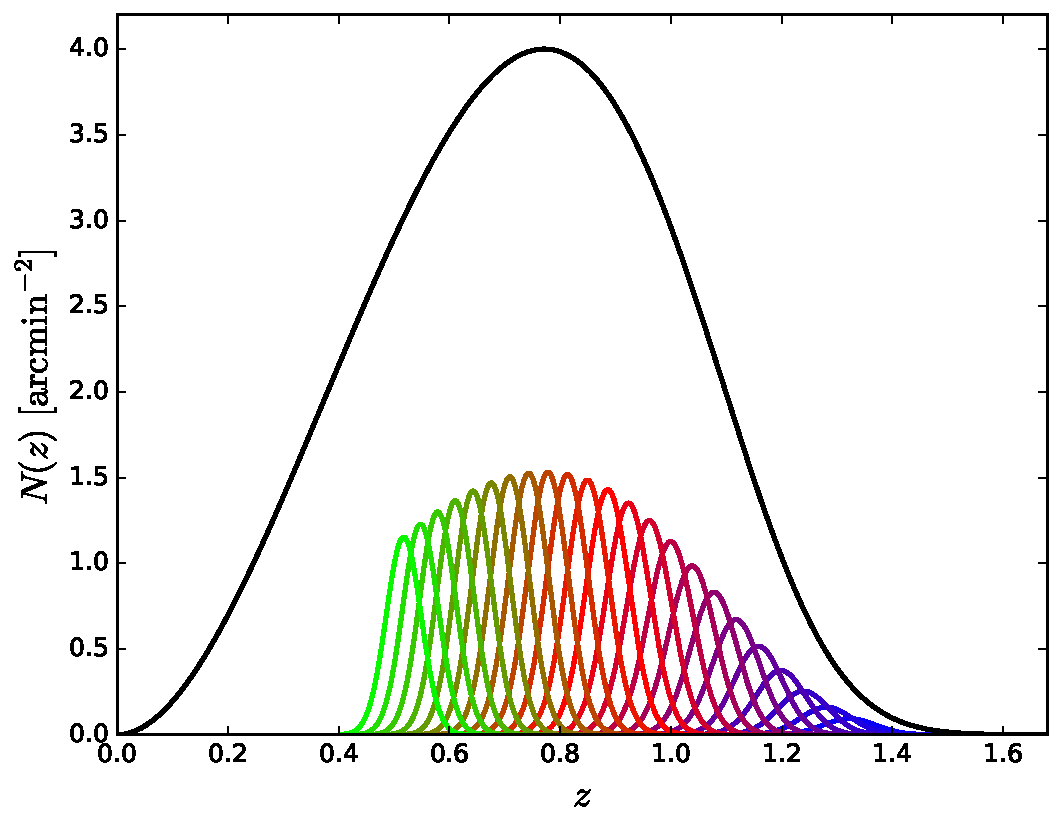
\includegraphics[width=0.49\textwidth]{Figs/nz_lsst_gc}
      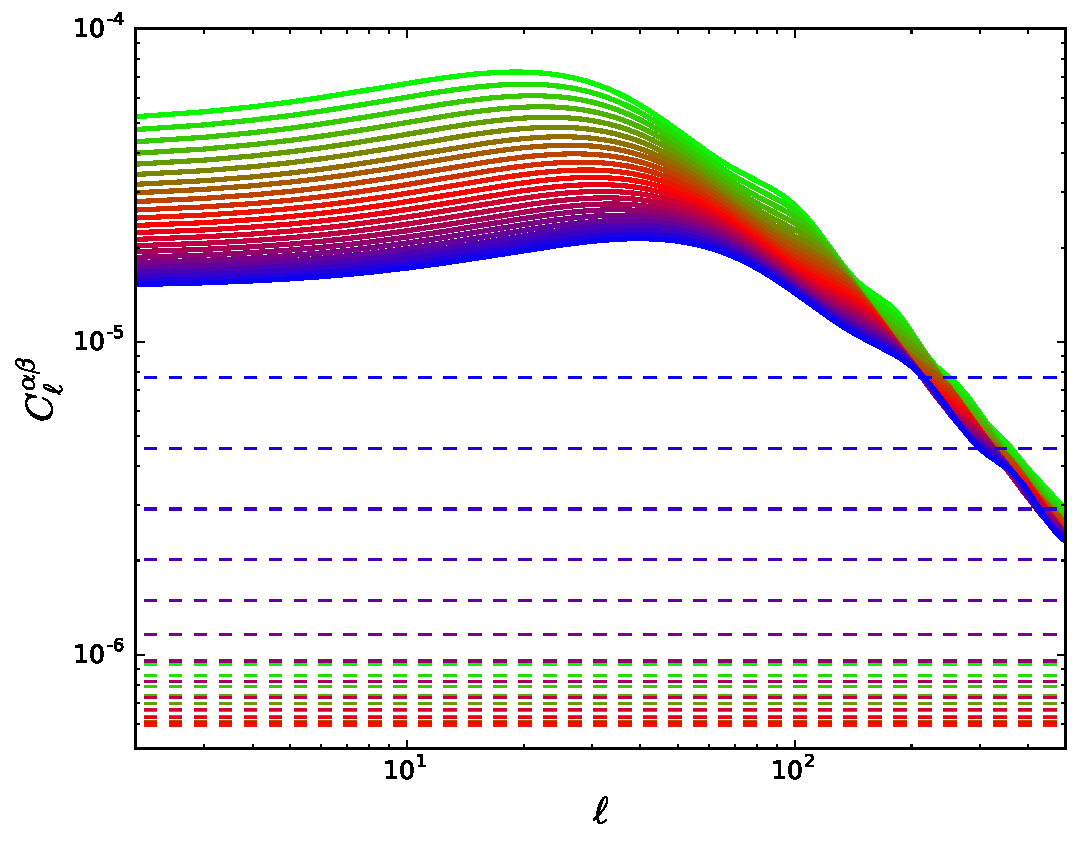
\includegraphics[width=0.49\textwidth]{Figs/c_ij_gc}
      \caption{{\sl Left}: redshift distribution and bins considered for the K-L analysis of a strawman large-scale-structure survey targeting a sample of red galaxies. {\sl Right}: clustering auto-power spectra of the redshift bins shown in the left panel. The signal and noise power spectra are shown as thick solid and thin dashed lines respectively.}\label{fig:nz_gc}
    \end{figure*}
    The assumptions used in the previous section are an ideal limit of the data collected by a photometric survey. In a more realistic (although still idealized) scenario, the information about the radial position of a given source is encoded in its posterior photo-$z$ distribution $p(z|\alpha)$, where $\alpha$ is a continuous variable determining the properties of the photo-$z$ (e.g. the mean of the posterior). The cross-power spectrum of two samples with photo-$z$ properties $\alpha$ and $\beta$ is given by
    \begin{align}
      &C_\ell^{\alpha\beta}=S^{\alpha\beta}_\ell+N^{\alpha\beta}_\ell,\\\label{eq:cl_generic}
      &S_\ell^{\alpha\beta}=\frac{2}{\pi}\int_0^\infty dk\,k^2\,\Delta_\ell^\alpha(k)\,\Delta_\ell^\beta(k),\\
      &N_\ell^{\alpha\beta}=\frac{\delta(\alpha-\beta)}{n_t\,p(\alpha)},
    \end{align}
    where $n_t$ is the total angular number density of sources,
    \begin{align}\nonumber
      &\Delta^{\alpha}_\ell(k)\equiv\int dz\,p(z|\alpha)\,\Psi_\ell(k,z)\,\sqrt{P(k,z)},\\\label{eq:tgc_dr}
      &\Psi_\ell(k,z)=b^\alpha(z)j_\ell(k\,\chi(z))-f(z)j_\ell''(k\,\chi(z)).
    \end{align}
    Here $b^\alpha(z)$ is the linear galaxy bias, $f(z)=d\log\delta/d\log a$ is the growth rate of structure, $P(k,z)$ is the matter power spectrum at redshift $z$, $p(\alpha)$ is the probability that a source has photo-$z$ properties $\alpha$, and $p(z|\alpha)$ is the conditional redshift distribution of these sources (we have labelled this quantity $\phi^\alpha(z)$ in previous sections). Note that, for simplicity, we have kept the contribution of redshift-space distortions at linear order and neglected the effect of magnification (this will be studied in Section REF).
    
    For a continuous variable $\alpha$, the generalized eigenvalue problem in Eq. \ref{eq:kl_sn} becomes a homogeneous Fredholm integral equation of the second kind:
    \begin{align}
      \int d\beta\,C^{\alpha\beta}_\ell e^p_\ell(\beta)=\lambda_p\int d\beta\,N^{\alpha\beta}_\ell e^p_\ell(\beta)\Rightarrow\\
      \Rightarrow\int d\beta\,n_t\,p(\alpha) S^{\alpha\beta}_\ell\,e^p_\ell(\beta)=(\lambda_p-1)e^p_\ell(\alpha).
    \end{align}
    In the limit of perfect photo-$z$ ($p(z|\alpha)=\delta(z-\alpha)$), and in the absence of redshift-space distortions, the solution to this equation are the spherical Bessel functions, as proven in the previous section. For general kernels, however, no analytical solution to the homogeneous Fredholm equation can usually be found, and the standard procedure to solve it is through discretization, which is equivalent to taking finite bins in $\alpha$. We will use this method here to find the K-L eigenmodes that maximize the signal content for galaxy clustering.

    To do so, we have considered a specific strawman photometric survey targeting a sample of red galaxies, characterized by their higher bias and better photo-$z$ uncertainties than their blue counterparts (and therefore better suited for clustering analyses). The sample we consider is compatible with what could be observed by LSST, characterized by the redshift distribution shown in the left panel of Fig. \ref{fig:nz_gc} (full details can be found in \cite{2015ApJ...814..145A}). We assume a photo-$z$ uncertainty of $\sigma_z=0.02\,(1+z)$ and split the sample into redshift bins in photo-$z$ space with $z_{\rm ph}>0.5$ and a width given by the photo-$z$ uncertainty at the bin centre. The auto-power spectra for our set of 23 bins are shown in the right panel of Fig. \ref{fig:nz_gc}. The large overlap between bins implies that a choice of thinner slices is unlikely to unveil significantly more information, and we have verified that the results shown below do not change after doubling the number of bins. 
    \begin{figure}
      \centering
      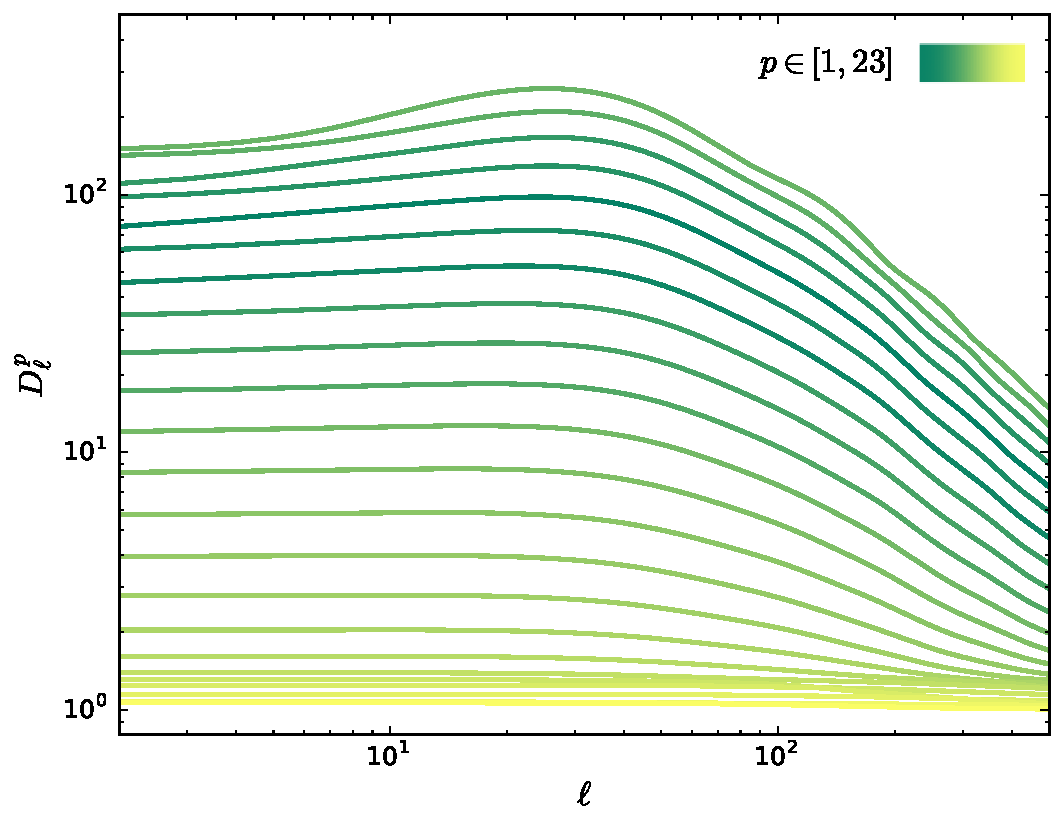
\includegraphics[width=0.49\textwidth]{Figs/d_p_gc}
      \caption{Power spectra of the K-L eigenmodes for the strawman weak large-scale-structure survey. Unlike in the case of weak lensing, a large number of eigenmodes are signal-dominated. This is due to the overall higher signal-to-noise ratio of galaxy clustering with respect to galaxy shear as well as to the smaller correlations between distant bins.}\label{fig:dp_gc}
    \end{figure}
    \begin{figure}
      \centering
      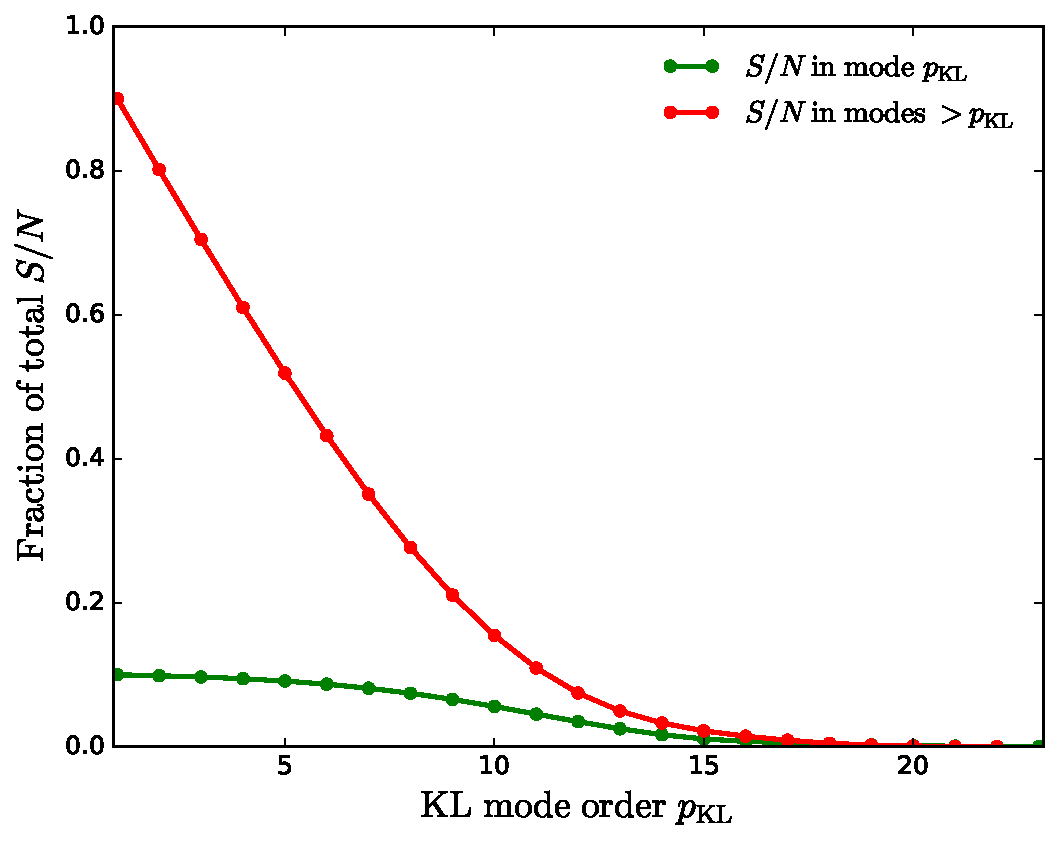
\includegraphics[width=0.49\textwidth]{Figs/information_gc}
      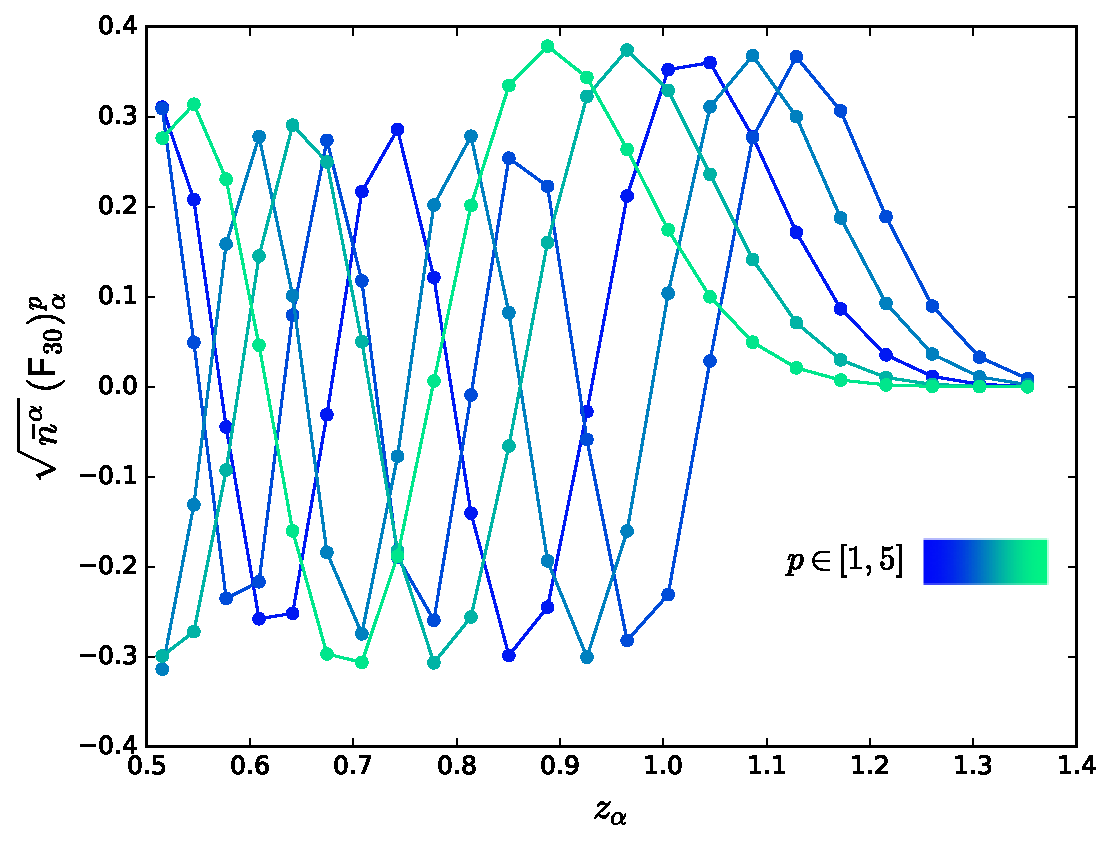
\includegraphics[width=0.49\textwidth]{Figs/kl_modes_gc}
      \caption{{\sl Left}: information content of the different K-L eigenmodes for the strawman galaxy clustering survey. The bulk of the information ($>90\%$) on $f_{\rm NL}$ is encoded in the first 12 modes. {\sl Left}: the first 5 K-L modes for $\ell=30$. The sinusoidal shape of the modes agrees with the expectation that, in the limit of $\sigma_z\rightarrow0$ and no background redshift dependence, the K-L modes should be given by the spherical Bessel functions. }\label{fig:kl_gc}
    \end{figure}    

    Using the prescription described in Section \ref{ssec:method.klbasis}, we find the K-L eigenmodes and associated power spectra, and rank them according to their contribution to the total signal-to-noise ratio (defined here as the Fisher matrix element of the signal amplitude). The power spectra of the resulting K-L modes are shown in Figure \ref{fig:dp_gc}. Unlike the case of weak lensing, explored in Section \ref{ssec:results.wl}, the information encoded in the galaxy overdensity is local in redshift, and thus the correlation between different bins decays rapidly with redshift separation. The signal-to-noise is therefore spread over $\sim15$ signal-dominated modes, and the noise-dominated modes can be thought of as the radial scales filtered out by the finite photo-$z$ uncertainty (as we mentioned in Section \ref{sssec:method.klbasis.sn}, the noise power spectrum gets mapped into $1$ under the K-L transform). The relative contribution of each mode to the total signal-to-noise is shown in the top panel of Fig. \ref{fig:kl_gc}. 90\% of the total constraining power can be achieved by considering the first 13 eigenvectors. The form of the first 7 of these eigenvectors for $\ell=30$ are shown in the right panel of Fig. \ref{fig:kl_gc}. The eigenmodes are sinusoids with increasing frequencies, in agreement with the expectation that, in the limit of $\sigma_z\rightarrow0$ and no background redshift dependence, the K-L decomposition is achieved by the spherical Bessel functions. A Fourier-Bessel decomposition is therefore probably a near-optimal analysis method, although the K-L decomposition allows a more precise determination of the truly orthogonal radial modes.
    
  \subsection{Galaxy clustering - optimal basis for $f_{\rm NL}$}\label{ssec:results.fnl}
    \begin{figure}
      \centering
      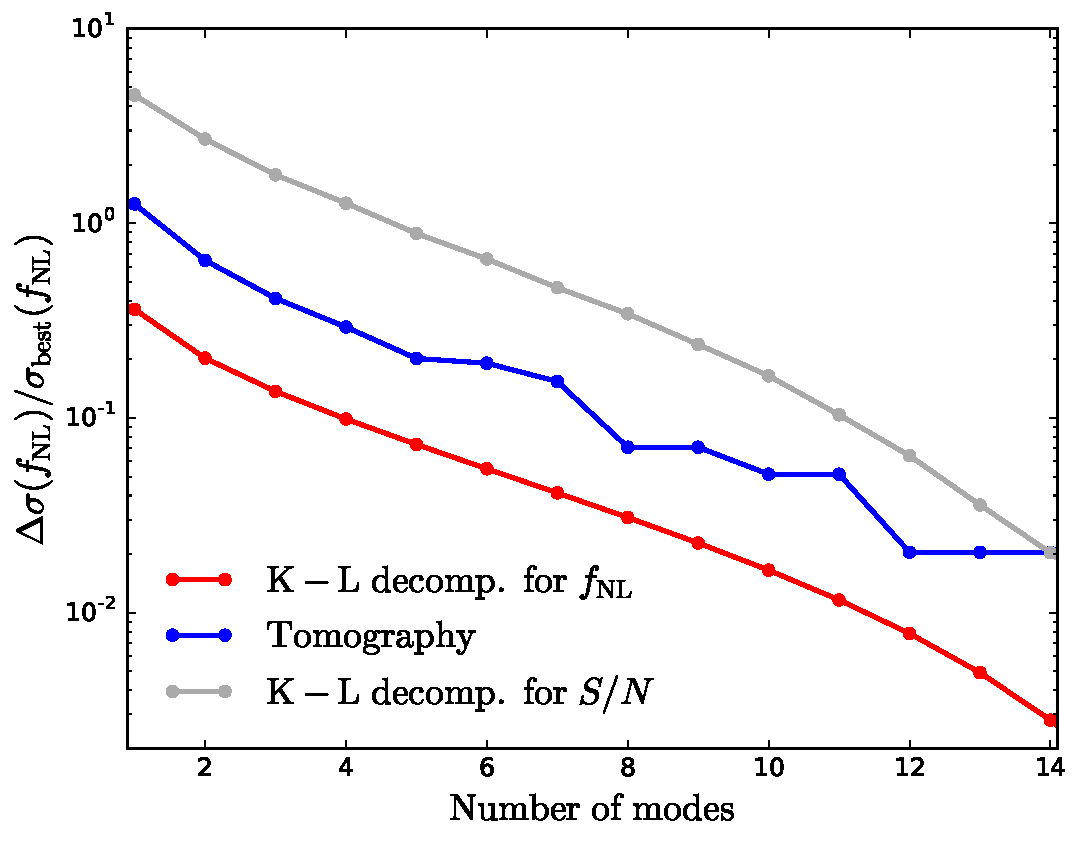
\includegraphics[width=0.49\textwidth]{Figs/kl_fnl}
      \caption{{\sl Left}: redshift distribution and bins considered for the K-L analysis of a strawman lensing survey}\label{fig:kl_fnl}
    \end{figure}
    It is expected that future large-scale photometric surveys will make the search for primordial non-Gaussianity one of their main science cases. This can be achieved by measuring the excess power on large scales caused by a non-zero value of $f_{\rm NL}$\footnote{The reader is referred to CITES for a thorough review of non-Gaussianity and a definition of $f_{\rm NL}$.} generates in the two-point statistics of biased tracers of the matter distribution CITES. Since the signal is most relevant on large scales, we can expect the bulk of it to be concentrated in a small number of radial modes, which makes the general K-L decomposition outlined in Section \ref{ssec:method.klbasis} an ideal analysis method. Similar approaches have been explored in the literature to devise optimal weights for spectroscopic galaxy surveys CITE.
    
    We again consider the red galaxy sample used in the previous section, but now estimate the K-L basis of eigenmodes that optimize the information content on $f_{\rm NL}$ instead of the overall signal amplitude. I.e. we solve the generalized eigenvalue problem in Eq. \ref{eq:kl_general} where $\theta=f_{\rm NL}$. We compare the performance of this basis with other choices of radial modes as follows: for a given number of modes, we estimate the associated uncertainty on $f_{\rm NL}$, $\sigma(f_{\rm NL})$ by summing the contributions to the corresponding Fisher matrix element of those modes, and compute the excess of $\sigma(f_{\rm NL})$ with respect to the best achievable constraint $\sigma_{\rm best}(f_{\rm NL})$. The results are shown in Fig. \ref{fig:kl_fnl} for three choices of radial functions:
    \begin{itemize}
      \item The K-L eigenbasis resulting from optimizing the information content on $f_{\rm NL}$ discussed in this section. The results are shown in red.
      \item The K-L eigenbasis resulting from optimizing the overall signal-to-noise of the galaxy clustering signal, as discussed in the previous section. The results are shown in gray.
      \item Photo-$z$ tomography: the result of dividing the galaxy sample into a number of top-hat photo-$z$ bins of equal width. The results are shown in blue.
    \end{itemize}
    As demonstrated by this Figure, for a fixed number of modes the optimal K-L basis always outperforms any other data compression prescription. In particular, the constraints on $f_{\rm NL}$ are only degraded by $\sim30\%$ when considering only the first principal eigenmode, and almost 90\% of the total constraining power is contained in the first three. Interestingly, a naive tomographic approach achieves the same uncertainty on $f_{\rm NL}$ with a smaller number of modes (redshift bins) than the K-L eigenbasis for the $S/N$. However, since the tomographic bins are not orthogonal, unlike the K-L modes, for a fixed $\sigma(f_{\rm NL})$ both K-L bases typically outperform the tomographic approach in terms of the size of the associated power spectrum. In any case, this example serves to stress the fact that the optimal radial basis in terms of overal $S/N$ is not necessary optimal in terms of final constraints for cosmological parameters that depend on specific features of the power spectrum.
    
  \subsection{Galaxy clustering - magnification bias}\label{ssec:results.mag}  
    \begin{figure}
      \centering
      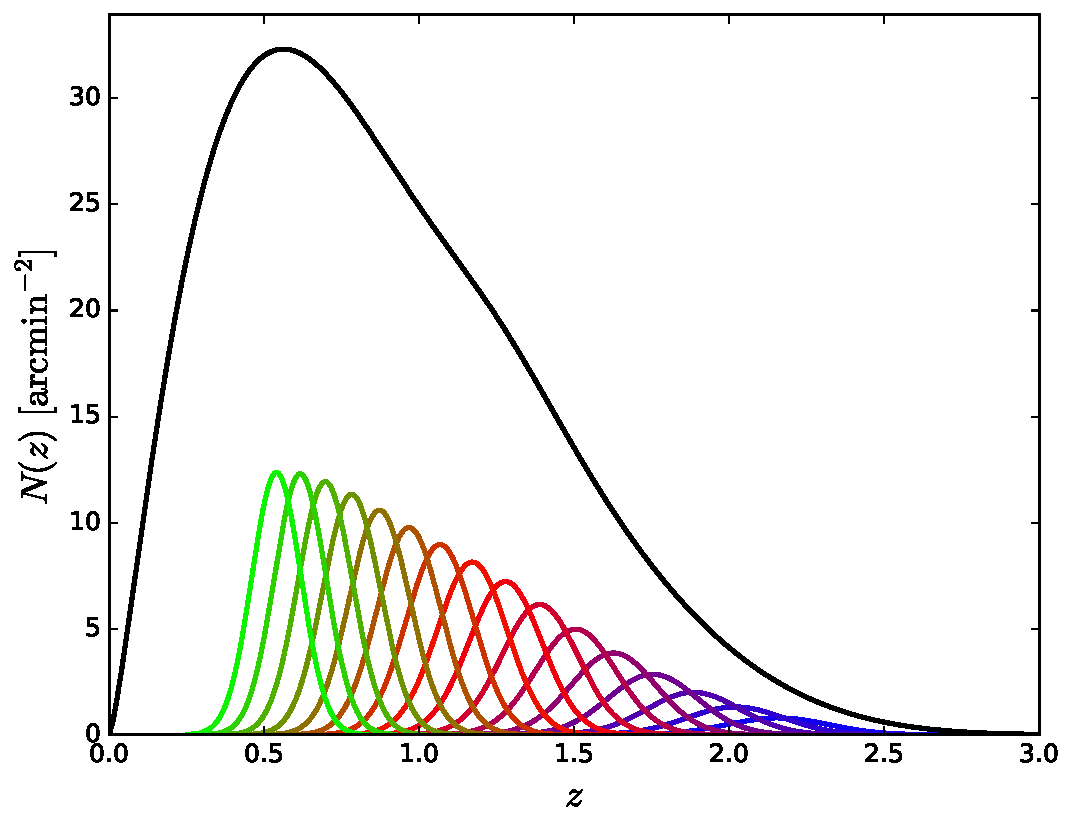
\includegraphics[width=0.49\textwidth]{Figs/nz_lsst_wl}
      \caption{{\sl Left}: redshift distribution and bins considered for the K-L analysis of a strawman lensing survey}\label{fig:nz_mb}
    \end{figure}
    \begin{figure}
      \centering
      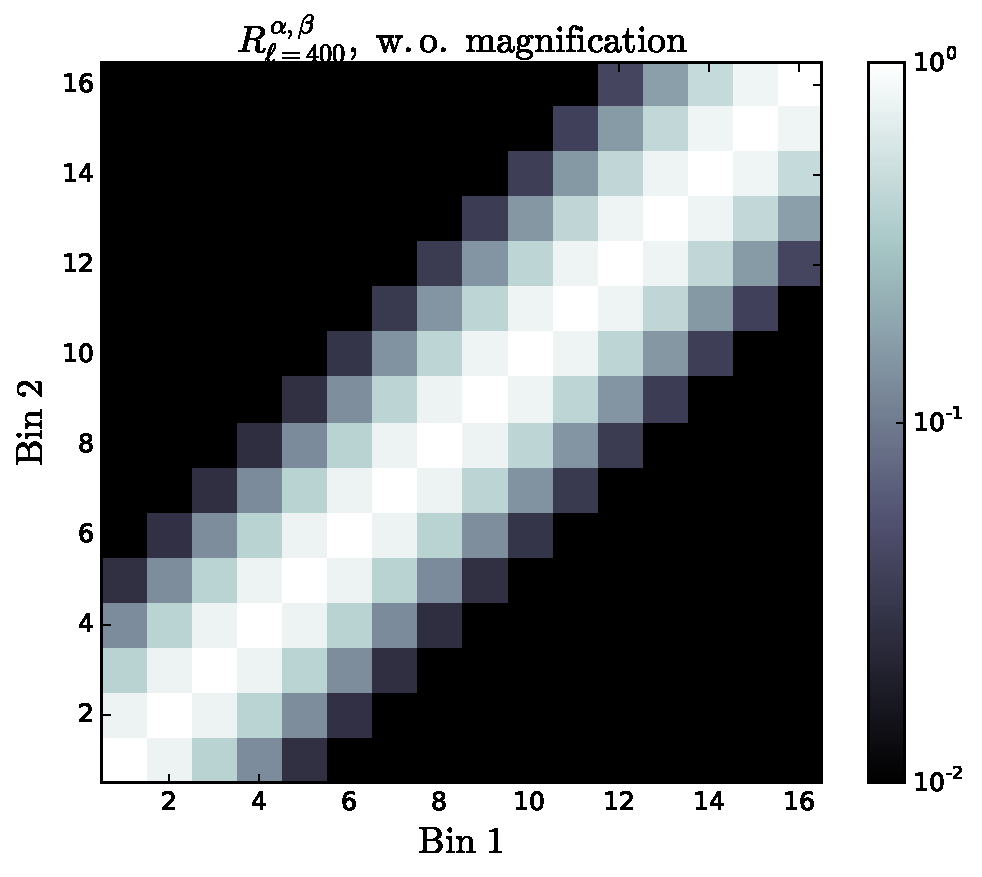
\includegraphics[width=0.49\textwidth]{Figs/r_ij_mb_wom}
      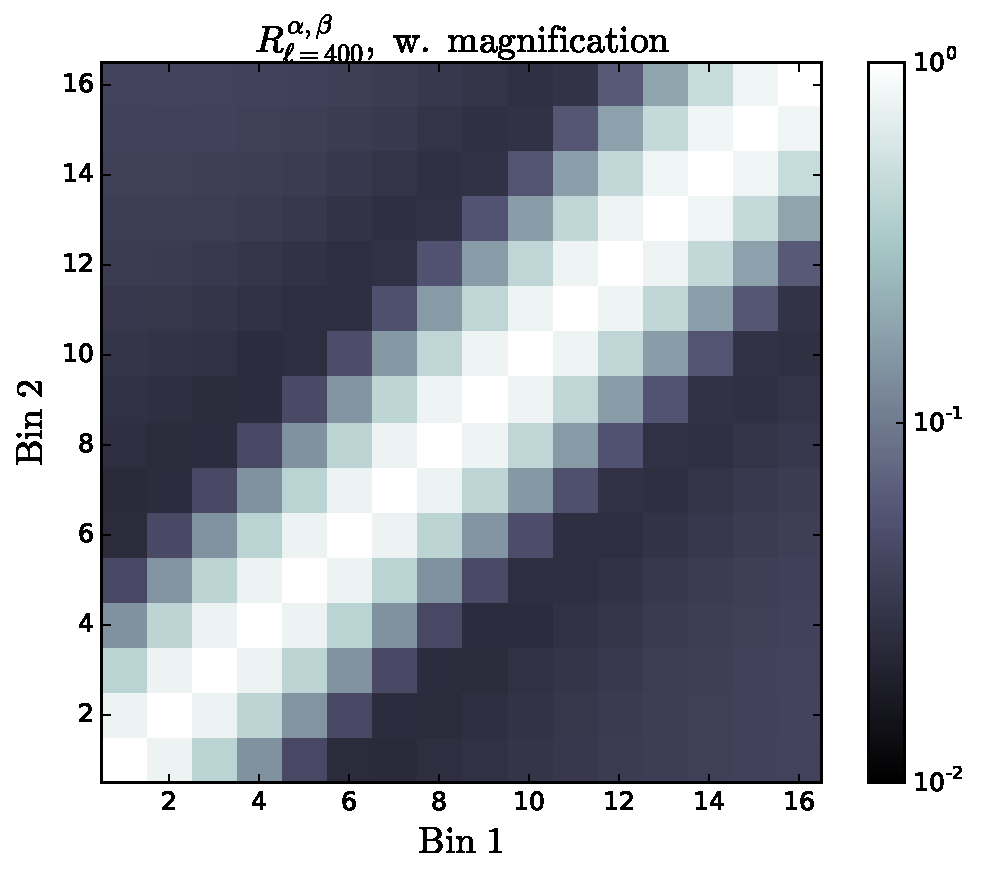
\includegraphics[width=0.49\textwidth]{Figs/r_ij_mb_wm}
      \caption{{\sl Left}: information content of the different K-L eigenmodes for the strawman galaxy clustering survey. The bulk of the information ($>90\%$) on $f_{\rm NL}$ is encoded in the first 12 modes. {\sl Left}: the first 5 K-L modes for $\ell=30$. The sinusoidal shape of the modes agrees with the expectation that, in the limit of $\sigma_z\rightarrow0$ and no background redshift dependence, the K-L modes should be given by the spherical Bessel functions. }\label{fig:r_ij_wm}
    \end{figure}
    \begin{figure}
      \centering
      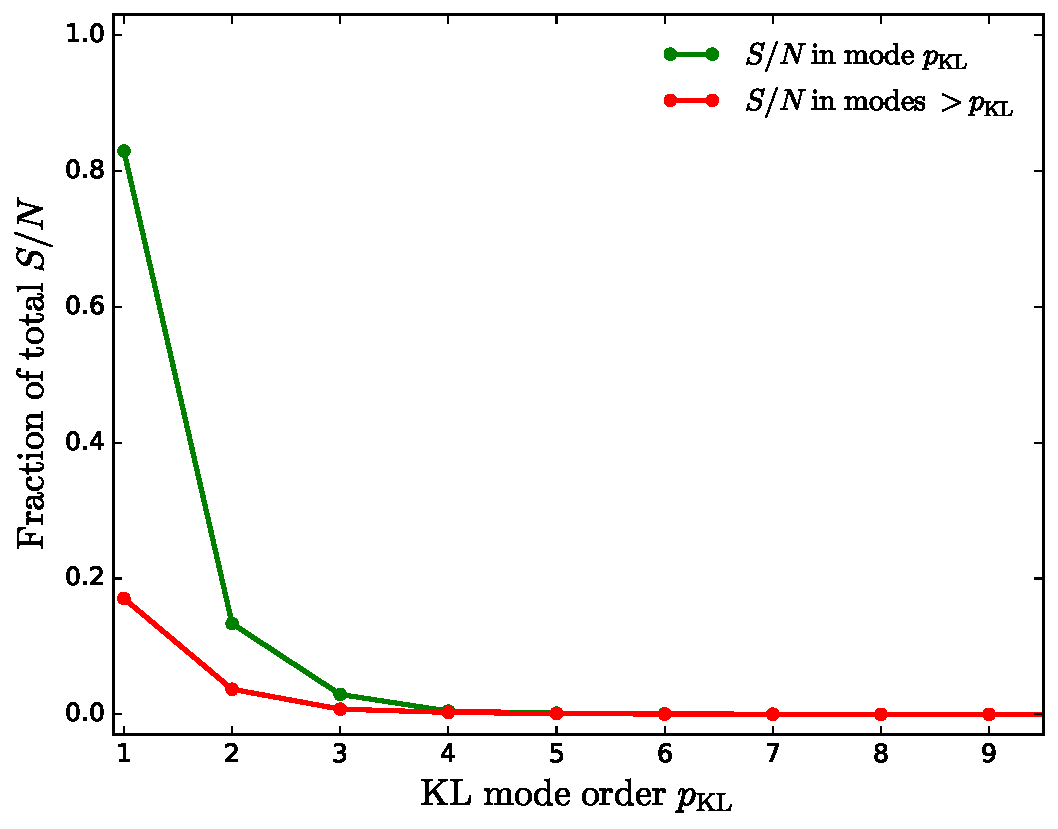
\includegraphics[width=0.49\textwidth]{Figs/information_mb}
      \caption{{\sl Left}: information content of the different K-L eigenmodes for the strawman galaxy clustering survey. The bulk of the information ($>90\%$) on $f_{\rm NL}$ is encoded in the first 12 modes. {\sl Left}: the first 5 K-L modes for $\ell=30$. The sinusoidal shape of the modes agrees with the expectation that, in the limit of $\sigma_z\rightarrow0$ and no background redshift dependence, the K-L modes should be given by the spherical Bessel functions. }\label{fig:kl_mb}
    \end{figure}
    Gravitational lensing of the galaxy positions alters the clustering pattern of galaxies through the so-called magnification bias effect. This appears as an extra term in the galaxy clustering transfer function (Eq. \ref{eq:tgc_dr}):
    \begin{align}\nonumber
      &\Delta^{M,\alpha}_\ell(k)=-2\ell(\ell+1)\int\,d\chi W^{M,\alpha}(\chi)\frac{j_\ell(k\chi)}{k^2a(\chi)}\sqrt{P(k,z(\chi))},\\
      &W^{M,\alpha}(\chi)=\frac{3H_0^2\Omega_M}{2}\int_{z(\chi)}^\infty dz'\,\phi^\alpha(z')\frac{2-5\,s}{2}\,\frac{\chi(z')-\chi}{\chi(z')\chi},
    \end{align}
    where $s$ is the tilt in the number counts of sources as a function of magnitude limit. This effect, commonly labeled ``magnification bias'' \cite{1967ApJ...147...61G,2000ApJ...537L..77M,2008PhRvD..77b3512L}, can be used as an alternative measurement of gravitational lensing, through galaxy positions instead of shapes. The contribution of the magnification term is, however, weak in comparison with the density and RSD terms (Eq. \ref{eq:tgc_dr}), and therefore its measurement can be hampered by the cosmic variance contribution of these terms.
    
    One can therefore think of the density and RSD terms as correlated contaminants of the magnification signal, and use the K-L formalism described in Section \ref{sssec:method.klbasis.cr} to devise an optimal basis of radial eigenmodes containing the bulk of its signal-to-noise.
    
    To test this approach we consider, as in the previous section, an LSST-like survey.  Since lensing magnification is an integrated effect, it is less hampered by poor photo-$z$ uncertainties, and it is most easily measured by cross-correlating high-redshift and low-redshift data CITES. For this reason, in this case we consider a sample of blue galaxies, with inferior photo-$z$ errors but wider redshift support. Full details can be found in \cite{2015ApJ...814..145A}. In summary, we consider a sample with $\sim40$ objects per arcmin$^2$ with the redshift distribution shown in Figure \ref{fig:nz_mb}. We also approximate the photo-$z$ distributions as Gaussians with a scatter $\sigma_z=0.05(1+z)$, and divide the sample into 16 top-hat bins in photo-$z$ space with $z_{\rm ph}<0.5$ and widths given by the value of $\sigma_z$ at the bin center (again, we verified that our conclusions did not change after decreasing the width by a factor 2).
    
    A key property of the magnification bias effect is the fact that, since gravitational lensing is caused by the integrated matter distribution between source and observer, the magnification signals in widely separated redshift bins can be tightly correlated. This is shown explicitly in Figure \ref{fig:r_ij_wm}. The figure shows the correlation coefficients between the 16 redshift bins, defined as $R^{\alpha\beta}_\ell=C^{\alpha\beta}_\ell/\sqrt{C^{\alpha\alpha}_\ell C^{\beta\beta}_\ell}$, at $\ell=400$, with (right panel) and without (left panel) the magnification bias effect. Although the contribution of lensing magnification to the correlation between neighbouring bins is subdominant, it produces noticeable correlations between distant ones.
    
    This property is particularly interesting in the context of the K-L decomposition: a signal that is tightly correlated accross samples will contribute significantly only to a small set of eigenmodes. To explore this possibility, we follow the prescription outlined in Section \ref{sssec:method.klbasis.cr} for correlated contaminants. The contribution of each eigenmode to the total signal-to-noise of the magnification bias (in a Fisher-matrix sense) is shown in Figure \ref{fig:kl_mb}. As expected, most of the signal ($>80\%$) is contained in the first eigenvalue, with the practical totality of it concetrated in the first three modes.
    
    We finish this section by noting that this approach is similar to the ``nulling'' method of \cite{2011MNRAS.415.1681H}, and that an analogous treatment could be carried out on the cosmic shear field to separate the lensing and intrinsic alignment contributions \cite{2008A&A...488..829J}.


  \subsection{Weak lensing - K-L basis for dark energy}\label{ssec:results.wl}
    \begin{figure}
      \centering
      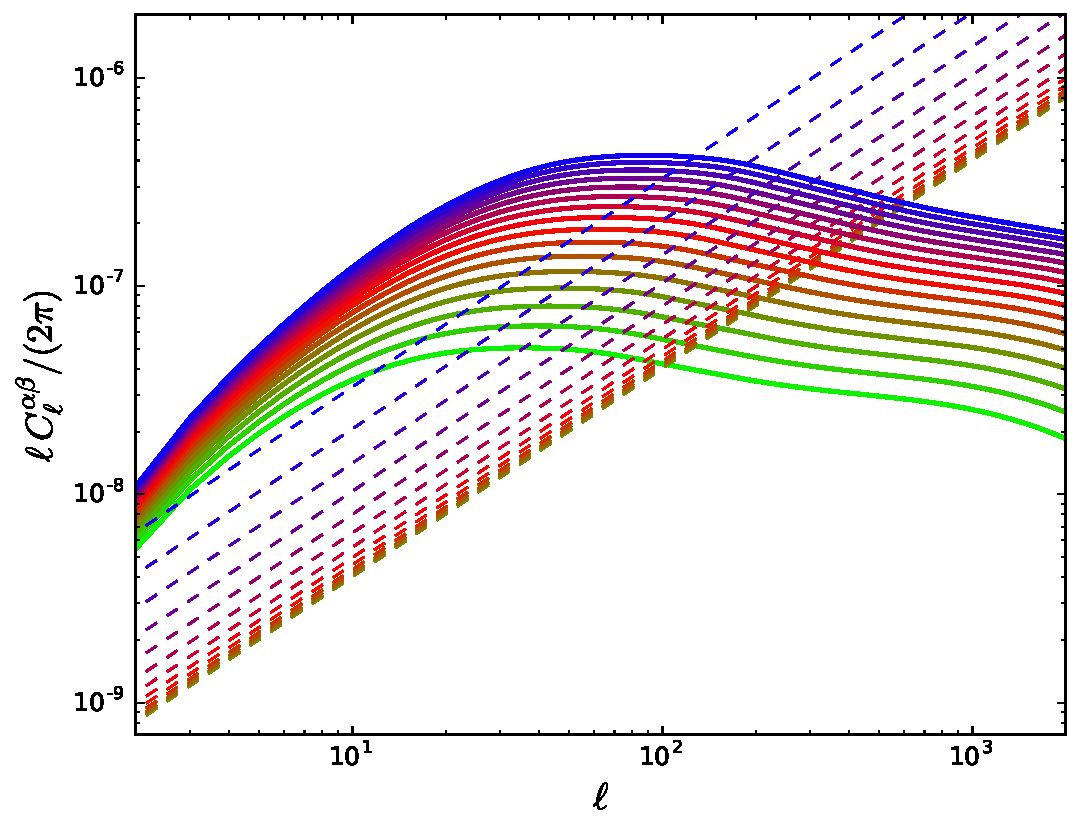
\includegraphics[width=0.49\textwidth]{Figs/c_ij_wl}
      \caption{Shear auto-power spectra of the redshift bins shown in the left panel. The signal and noise power spectra are shown as thick solid and thin dashed lines respectively.}\label{fig:nz_wl}
    \end{figure}
    \begin{figure}
      \centering
      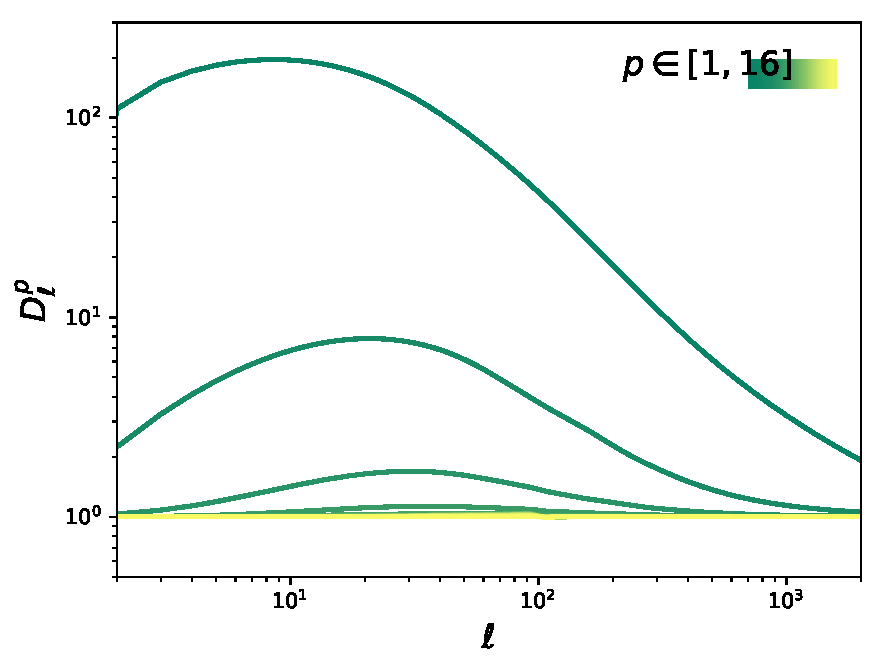
\includegraphics[width=0.49\textwidth]{Figs/d_p_wl}
      \caption{Power spectra of the K-L eigenmodes for the strawman weak lensing survey. All but the first three modes are noise-dominated, and most of the information is encoded in the first mode.}\label{fig:dp_wl}
    \end{figure}
    \begin{figure*}
      \centering
      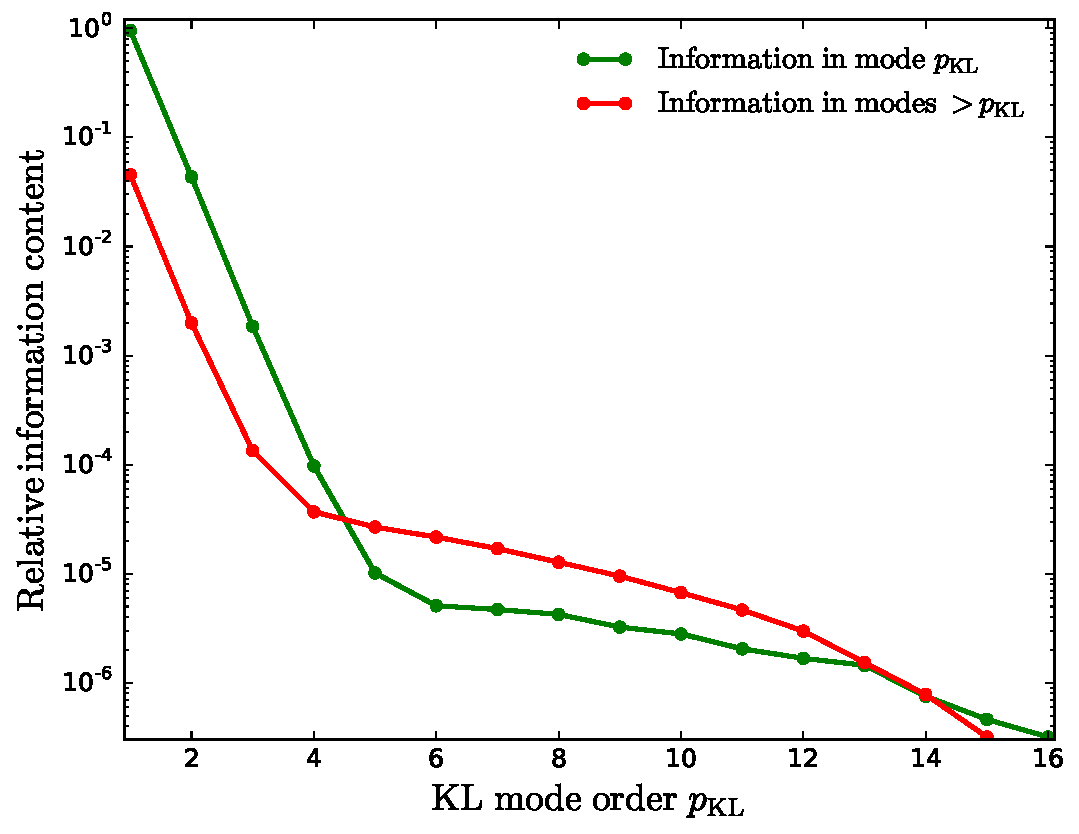
\includegraphics[width=0.49\textwidth]{Figs/information_wl}
      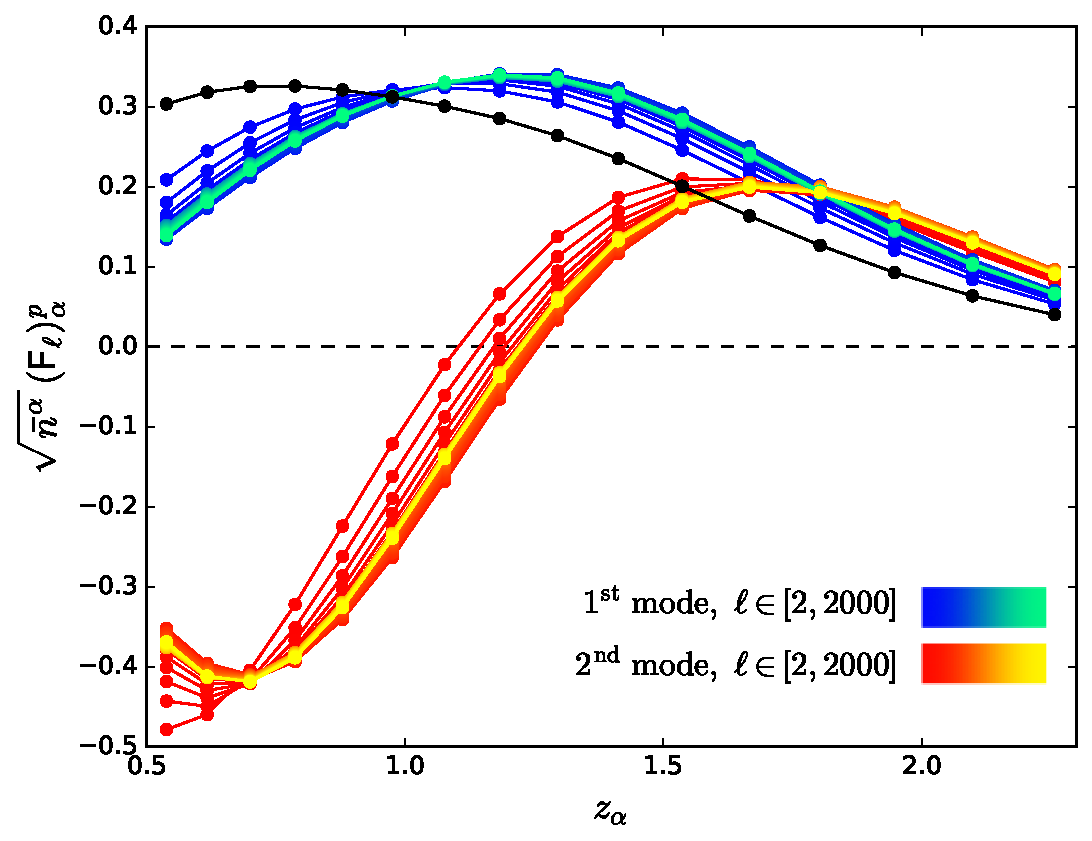
\includegraphics[width=0.49\textwidth]{Figs/kl_modes_wl}
      \caption{{\sl Left}: the first (blue-cyan) and second (red-yellow) eigenmodes of the strawman weak-lensing survey for different $\ell$. The redshift dependence of the modes stays roughly constant across $\ell$ and converges to a fixed shape for large $\ell$. {\sl Right}: information content of the different eigenmodes. Most of the information $\sim95\%$ is encoded in the first bin, and more than $99\%$ of it can be recovered considering only the first 2 modes.}\label{fig:kl_wl}
    \end{figure*}
    The effects of gravitational lensing can be measured directly by studying the correlation it induces on the shapes and orientation of galaxy images. This effect, labeled ``cosmic shear'' is arguably the most promising observational probe for photometric redshift surveys, and therefore we will discuss the K-L analysis of this signal in particular detail.
    
    As in the case of lensing magnification, and unlike the dominant galaxy clustering terms, the cosmic shear signal is correlated between widely separated redshift bins due to the integrated nature of gravitational lensing. Thus we can expect that a K-L transform should be able to compress most of the signal to noise into a small set of radial eigenmodes. To quantify this mothed we consider the same survey configuration used in Section \ref{ssec:results.mag}. The signal part of the cross-power spectrum between the cosmic shear measurements made in two different redshift shells is given again by Eq. \ref{eq:cl_generic}, where now the transfer functions $\Delta^{\alpha}_\ell$ take the form:
    \begin{align}\nonumber
      &\Delta^{\alpha}_\ell(k)\equiv\sqrt{\frac{(\ell+2)!}{(\ell-2)!}}\int d\chi\,W^\alpha(\chi)\frac{j_\ell(k\chi)}{k^2a(\chi)}\sqrt{P(k,z(\chi))},\\%\hspace{12pt}
      &W^\alpha(\chi)\equiv\frac{3H_0^2\Omega_M}{2}\int_{z(\chi)}^\infty dz\,\phi^\alpha(z')\frac{\chi(z')-\chi}{\chi(z')\chi}.
    \end{align}
    The noise power spectrum is white and simply given by the intrinsic ellipticity scatter weighed by the angular number density of sources in each redshift bin $\bar{n}^\alpha$:
    \begin{equation}
      N^{\alpha\beta}_\ell=\delta_{\alpha\beta}\frac{\sigma_\gamma^2}{\bar{n}^\alpha},
    \end{equation}
    with $\bar{n}^\alpha$ in units of ${\rm srad}^{-1}$. We use $\sigma_\gamma=0.28$. The lensing auto-power spectra (both signal and noise) for these bins are shown in Figure \ref{fig:nz_wl}.
    
    We compute the K-L modes for this setup and rank them according to their contribution to the total lensing signal (in a Fisher matrix sense). The power spectra of the resulting set of modes are shown in the left panel of Figure \ref{fig:dp_wl}. Comparing against Fig. \ref{fig:nz_wl} we can see that the K-L decomposition effectively separates the signal-dominated and noise-dominated modes, with all modes $p>3$ dominated by noise. The fractional contribution of each mode to the total signal-to-noise is shown in the left panel of Figure \ref{fig:kl_wl}. Most of the signal ($\sim95\%$) is contained within a single mode, and the first two modes are able to recover more than $99\%$ of the total. The eigenvectors corresponding to the first three principal modes for different values of $\ell$ are shown in the right panel of the same figure. We observe that the eigenvectors preserve roughly the same shape for all $\ell$, and converge to the same shape at large $\ell$. The first eigenvector upweights the parts of the redshift range with the highest signal-to-noise, penalising the low-$z$ regime due to its poor lensing signal and the high-$z$ bins due to their high shot noise. The second and third eigenmodes then recover part of this information by marginally upweighting these regions.
    
    Since the cosmological lensing signal at a given redshift $z$ is caused by matter distribution at all redshifts $<z$, different redshift bins are tightly correlated at the signal level. This is the main reason for the large degree of data compression achievable in this case, a  statement that is in principle largely independent of the properties of the photometric redshifts. Exploiting this property could therefore significantly simplify the analysis of weak lensing datasets.
    
\section{Practical example: weak lensing}
  \lipsum[2]

\section{Discussion}\label{sec:discussion}
  \lipsum[3]
  
  open problems: contaminant deprojection, mode coupling from incomplete sky, IA in single-mode lensing
  
  
\section*{Acknowledgements}
  \lipsum[4]
  
\bibliography{paper}

\appendix
\onecolumngrid
\section{Pseudo-$C_\ell$ estimation of the K-L modes}\label{app:pcl}
  One of the standard methods to estimate the angular power spectrum of any two quantities in the cut sky is the so-called pseudo-$C_\ell$ estimator. This section adapts this method to the modes resulting from the K-L decomposition described before.
  
  The standard pseudo-$C_\ell$ method is based on computing the spherical harmonic coefficients of the mask field:
  \begin{equation}
    \tilde{a}^\alpha_{\ell m}=\int d\nv\,a^\alpha(\nv)\,w^\alpha(\nv),
  \end{equation}
  where $w^\alpha$ is the weights map characterizing the mask of the field $a^\alpha$. One then estimates the power spectrum of this object by averaging over $m$ for each $\ell$:
  \begin{equation}
    \tilde{C}^{\alpha\beta}_\ell\equiv\frac{\sum_m\tilde{a}^\alpha_{\ell m}\tilde{a}^{\beta *}_{\ell m}}{2\ell+1}.
  \end{equation}
  This object is then related to the true underlying power spectrum through a mode-coupling matrix $M^{\alpha\beta}_{\ell\ell'}$ such that
  \begin{equation}
    \tilde{C}^{\alpha\beta}_\ell=\sum_{\ell'}M^{\alpha\beta}_{\ell\ell'}C^{\alpha\beta}_{\ell'},\hspace{12pt}
    M^{\alpha\beta}_{\ell \ell'}\equiv\sum_{\ell''}\frac{(2\ell'+1)(2\ell''+1)}{4\pi}W^{\alpha\beta}_{\ell''}
    \left(
    \begin{array}{ccc}
      \ell & \ell' & \ell''\\
      0 & 0 & 0
    \end{array}
    \right)^2
  \end{equation}
  where the coupling matrix $M$ depends solely on the power spectrum of the masks $W^{\alpha\beta}_\ell\equiv(2\ell+1)^{-1}\sum_mw^\alpha_{\ell m}w^{\beta *}_{\ell m}$.
  
  The extension of this estimator to the power spectrum of the K-L modes is straightforward: we project the masked harmonic coefficients $\tilde{a}^\alpha$ over the K-L eigenvectors ${\sf E}$ (i.e. $\tilde{\bf b}_{\ell m}\equiv {\sf E}_\ell\circ\tilde{\bf a}_{\ell m}$) and compute their power spectra by averaging over $m$. The resulting estimator takes the form $\tilde{D}^p_\ell=\sum_{\ell'}M_{\ell\ell'}^{pp'}D^{p'}_{\ell'}$, where the new mode-coupling matrix is given by:
  \begin{equation}
    M^{pp'}_{\ell\ell'}\equiv M^{\alpha\beta}_{\ell\ell'}\left[({\sf E}_\ell)^p_\alpha({\sf N}^{-1})_{\alpha\alpha'}({\sf E}_{\ell'})^{p'}_{\alpha'}\right]\left[({\sf E}_\ell)^p_\beta({\sf N}^{-1})_{\beta\beta'}({\sf E}_{\ell'})^{p'}_{\beta'}\right]
    =M_{\ell\ell'}\left[({\sf E}_\ell)^p_\alpha({\sf N}^{-1}_\ell)_{\alpha\beta}({\sf E}_{\ell'})^{p'}_\beta\right]^2
  \end{equation}
  where the second equality holds only if all the maps $a^\alpha_\ell$ share the same mask $w$.\footnote{Note that, for full-sky coverage $M_{\ell\ell'}=\delta_{\ell\ell'}$ and using the orthonormality of ${\sf E}$ we get $M^{pp'}_{\ell\ell'}=\delta_{\ell\ell'}\delta_{pp'}$.}
  
  \cite{2013arXiv1307.1307M,2015PhRvD..92l3010L}

\end{document}
